\documentclass[1p]{elsarticle_modified}
%\bibliographystyle{elsarticle-num}

%\usepackage[colorlinks]{hyperref}
%\usepackage{abbrmath_seonhwa} %\Abb, \Ascr, \Acal ,\Abf, \Afrak
\usepackage{amsfonts}
\usepackage{amssymb}
\usepackage{amsmath}
\usepackage{amsthm}
\usepackage{scalefnt}
\usepackage{amsbsy}
\usepackage{kotex}
\usepackage{caption}
\usepackage{subfig}
\usepackage{color}
\usepackage{graphicx}
\usepackage{xcolor} %% white, black, red, green, blue, cyan, magenta, yellow
\usepackage{float}
\usepackage{setspace}
\usepackage{hyperref}

\usepackage{tikz}
\usetikzlibrary{arrows}

\usepackage{multirow}
\usepackage{array} % fixed length table
\usepackage{hhline}

%%%%%%%%%%%%%%%%%%%%%
\makeatletter
\renewcommand*\env@matrix[1][\arraystretch]{%
	\edef\arraystretch{#1}%
	\hskip -\arraycolsep
	\let\@ifnextchar\new@ifnextchar
	\array{*\c@MaxMatrixCols c}}
\makeatother %https://tex.stackexchange.com/questions/14071/how-can-i-increase-the-line-spacing-in-a-matrix
%%%%%%%%%%%%%%%

\usepackage[normalem]{ulem}

\newcommand{\msout}[1]{\ifmmode\text{\sout{\ensuremath{#1}}}\else\sout{#1}\fi}
%SOURCE: \msout is \stkout macro in https://tex.stackexchange.com/questions/20609/strikeout-in-math-mode

\newcommand{\cancel}[1]{
	\ifmmode
	{\color{red}\msout{#1}}
	\else
	{\color{red}\sout{#1}}
	\fi
}

\newcommand{\add}[1]{
	{\color{blue}\uwave{#1}}
}

\newcommand{\replace}[2]{
	\ifmmode
	{\color{red}\msout{#1}}{\color{blue}\uwave{#2}}
	\else
	{\color{red}\sout{#1}}{\color{blue}\uwave{#2}}
	\fi
}

\newcommand{\Sol}{\mathcal{S}} %segment
\newcommand{\D}{D} %diagram
\newcommand{\A}{\mathcal{A}} %arc


%%%%%%%%%%%%%%%%%%%%%%%%%%%%%5 test

\def\sl{\operatorname{\textup{SL}}(2,\Cbb)}
\def\psl{\operatorname{\textup{PSL}}(2,\Cbb)}
\def\quan{\mkern 1mu \triangleright \mkern 1mu}

\theoremstyle{definition}
\newtheorem{thm}{Theorem}[section]
\newtheorem{prop}[thm]{Proposition}
\newtheorem{lem}[thm]{Lemma}
\newtheorem{ques}[thm]{Question}
\newtheorem{cor}[thm]{Corollary}
\newtheorem{defn}[thm]{Definition}
\newtheorem{exam}[thm]{Example}
\newtheorem{rmk}[thm]{Remark}
\newtheorem{alg}[thm]{Algorithm}

\newcommand{\I}{\sqrt{-1}}
\begin{document}

%\begin{frontmatter}
%
%\title{Boundary parabolic representations of knots up to 8 crossings}
%
%%% Group authors per affiliation:
%\author{Yunhi Cho} 
%\address{Department of Mathematics, University of Seoul, Seoul, Korea}
%\ead{yhcho@uos.ac.kr}
%
%
%\author{Seonhwa Kim} %\fnref{s_kim}}
%\address{Center for Geometry and Physics, Institute for Basic Science, Pohang, 37673, Korea}
%\ead{ryeona17@ibs.re.kr}
%
%\author{Hyuk Kim}
%\address{Department of Mathematical Sciences, Seoul National University, Seoul 08826, Korea}
%\ead{hyukkim@snu.ac.kr}
%
%\author{Seokbeom Yoon}
%\address{Department of Mathematical Sciences, Seoul National University, Seoul, 08826,  Korea}
%\ead{sbyoon15@snu.ac.kr}
%
%\begin{abstract}
%We find all boundary parabolic representation of knots up to 8 crossings.
%
%\end{abstract}
%\begin{keyword}
%    \MSC[2010] 57M25 
%\end{keyword}
%
%\end{frontmatter}

%\linenumbers
%\tableofcontents
%
\newcommand\colored[1]{\textcolor{white}{\rule[-0.35ex]{0.8em}{1.4ex}}\kern-0.8em\color{red} #1}%
%\newcommand\colored[1]{\textcolor{white}{ #1}\kern-2.17ex	\textcolor{white}{ #1}\kern-1.81ex	\textcolor{white}{ #1}\kern-2.15ex\color{red}#1	}

{\Large $\underline{11a_{256}~(K11a_{256})}$}

\setlength{\tabcolsep}{10pt}
\renewcommand{\arraystretch}{1.6}
\vspace{1cm}\begin{tabular}{m{100pt}>{\centering\arraybackslash}m{274pt}}
\multirow{5}{120pt}{
	\centering
	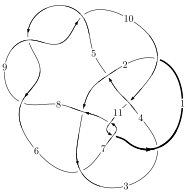
\includegraphics[width=112pt]{../../../GIT/diagram.site/Diagrams/png/505_11a_256.png}\\
\ \ \ A knot diagram\footnotemark}&
\allowdisplaybreaks
\textbf{Linearized knot diagam} \\
\cline{2-2}
 &
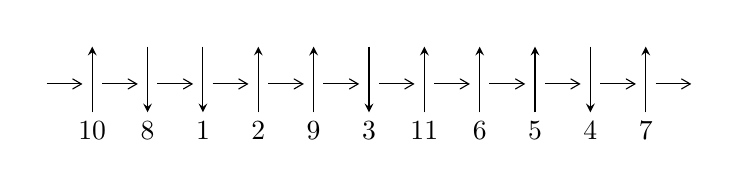
\begin{tikzpicture}[x=20pt, y=17pt]
	% nodes
	\node (C0) at (0, 0) {};
	\node (C1) at (1, 0) {};
	\node (C1U) at (1, +1) {};
	\node (C1D) at (1, -1) {10};

	\node (C2) at (2, 0) {};
	\node (C2U) at (2, +1) {};
	\node (C2D) at (2, -1) {8};

	\node (C3) at (3, 0) {};
	\node (C3U) at (3, +1) {};
	\node (C3D) at (3, -1) {1};

	\node (C4) at (4, 0) {};
	\node (C4U) at (4, +1) {};
	\node (C4D) at (4, -1) {2};

	\node (C5) at (5, 0) {};
	\node (C5U) at (5, +1) {};
	\node (C5D) at (5, -1) {9};

	\node (C6) at (6, 0) {};
	\node (C6U) at (6, +1) {};
	\node (C6D) at (6, -1) {3};

	\node (C7) at (7, 0) {};
	\node (C7U) at (7, +1) {};
	\node (C7D) at (7, -1) {11};

	\node (C8) at (8, 0) {};
	\node (C8U) at (8, +1) {};
	\node (C8D) at (8, -1) {6};

	\node (C9) at (9, 0) {};
	\node (C9U) at (9, +1) {};
	\node (C9D) at (9, -1) {5};

	\node (C10) at (10, 0) {};
	\node (C10U) at (10, +1) {};
	\node (C10D) at (10, -1) {4};

	\node (C11) at (11, 0) {};
	\node (C11U) at (11, +1) {};
	\node (C11D) at (11, -1) {7};
	\node (C12) at (12, 0) {};

	% arrows
	\draw[->,>={angle 60}]
	(C0) edge (C1) (C1) edge (C2) (C2) edge (C3) (C3) edge (C4) (C4) edge (C5) (C5) edge (C6) (C6) edge (C7) (C7) edge (C8) (C8) edge (C9) (C9) edge (C10) (C10) edge (C11) (C11) edge (C12) ;	\draw[->,>=stealth]
	(C1D) edge (C1U) (C2U) edge (C2D) (C3U) edge (C3D) (C4D) edge (C4U) (C5D) edge (C5U) (C6U) edge (C6D) (C7D) edge (C7U) (C8D) edge (C8U) (C9D) edge (C9U) (C10U) edge (C10D) (C11D) edge (C11U) ;
	\end{tikzpicture} \\
\hhline{~~} \\& 
\textbf{Solving Sequence} \\ \cline{2-2} 
 &
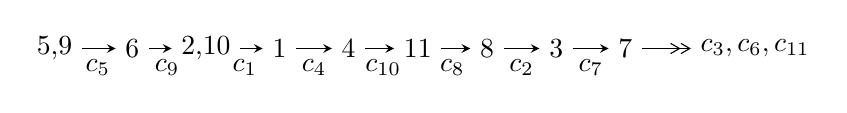
\begin{tikzpicture}[x=25pt, y=7pt]
	% node
	\node (A0) at (-1/8, 0) {5,9};
	\node (A1) at (1, 0) {6};
	\node (A2) at (33/16, 0) {2,10};
	\node (A3) at (25/8, 0) {1};
	\node (A4) at (33/8, 0) {4};
	\node (A5) at (41/8, 0) {11};
	\node (A6) at (49/8, 0) {8};
	\node (A7) at (57/8, 0) {3};
	\node (A8) at (65/8, 0) {7};
	\node (C1) at (1/2, -1) {$c_{5}$};
	\node (C2) at (3/2, -1) {$c_{9}$};
	\node (C3) at (21/8, -1) {$c_{1}$};
	\node (C4) at (29/8, -1) {$c_{4}$};
	\node (C5) at (37/8, -1) {$c_{10}$};
	\node (C6) at (45/8, -1) {$c_{8}$};
	\node (C7) at (53/8, -1) {$c_{2}$};
	\node (C8) at (61/8, -1) {$c_{7}$};
	\node (A9) at (10, 0) {$c_{3},c_{6},c_{11}$};

	% edge
	\draw[->,>=stealth]	
	(A0) edge (A1) (A1) edge (A2) (A2) edge (A3) (A3) edge (A4) (A4) edge (A5) (A5) edge (A6) (A6) edge (A7) (A7) edge (A8) ;
	\draw[->>,>={angle 60}]	
	(A8) edge (A9);
\end{tikzpicture} \\ 

\end{tabular} \\

\footnotetext{
The image of knot diagram is generated by the software ``\textbf{Draw programme}" developed by Andrew Bartholomew(\url{http://www.layer8.co.uk/maths/draw/index.htm\#Running-draw}), where we modified some parts for our purpose(\url{https://github.com/CATsTAILs/LinksPainter}).
}\phantom \\ \newline 
\centering \textbf{Ideals for irreducible components\footnotemark of $X_{\text{par}}$} 
 
\begin{align*}
I^u_{1}&=\langle 
-8.45189\times10^{122} u^{81}+2.24341\times10^{123} u^{80}+\cdots+2.70538\times10^{122} b+1.42226\times10^{122},\\
\phantom{I^u_{1}}&\phantom{= \langle  }8.78383\times10^{122} u^{81}-2.33856\times10^{123} u^{80}+\cdots+2.70538\times10^{122} a+1.70512\times10^{123},\;u^{82}-3 u^{81}+\cdots-15 u+1\rangle \\
I^u_{2}&=\langle 
- u^{14}-2 u^{13}-10 u^{12}-17 u^{11}-40 u^{10}-55 u^9-79 u^8-82 u^7-76 u^6-51 u^5-27 u^4-4 u^3+2 u^2+b+4 u,\\
\phantom{I^u_{2}}&\phantom{= \langle  }u^{15}+u^{14}+8 u^{13}+8 u^{12}+24 u^{11}+22 u^{10}+31 u^9+21 u^8+11 u^7-4 u^6-7 u^5-11 u^4+2 u^2+a+3 u+1,\\
\phantom{I^u_{2}}&\phantom{= \langle  }u^{16}+2 u^{15}+\cdots-4 u^2+1\rangle \\
\\
\end{align*}
\raggedright * 2 irreducible components of $\dim_{\mathbb{C}}=0$, with total 98 representations.\\
\footnotetext{All coefficients of polynomials are rational numbers. But the coefficients are sometimes approximated in decimal forms when there is not enough margin.}
\newpage
\renewcommand{\arraystretch}{1}
\centering \section*{I. $I^u_{1}= \langle -8.45\times10^{122} u^{81}+2.24\times10^{123} u^{80}+\cdots+2.71\times10^{122} b+1.42\times10^{122},\;8.78\times10^{122} u^{81}-2.34\times10^{123} u^{80}+\cdots+2.71\times10^{122} a+1.71\times10^{123},\;u^{82}-3 u^{81}+\cdots-15 u+1 \rangle$}
\flushleft \textbf{(i) Arc colorings}\\
\begin{tabular}{m{7pt} m{180pt} m{7pt} m{180pt} }
\flushright $a_{5}=$&$\begin{pmatrix}1\\0\end{pmatrix}$ \\
\flushright $a_{9}=$&$\begin{pmatrix}0\\u\end{pmatrix}$ \\
\flushright $a_{6}=$&$\begin{pmatrix}1\\- u^2\end{pmatrix}$ \\
\flushright $a_{2}=$&$\begin{pmatrix}-3.24680 u^{81}+8.64413 u^{80}+\cdots+21.7051 u-6.30272\\3.12411 u^{81}-8.29242 u^{80}+\cdots+33.1864 u-0.525715\end{pmatrix}$ \\
\flushright $a_{10}=$&$\begin{pmatrix}u\\u\end{pmatrix}$ \\
\flushright $a_{1}=$&$\begin{pmatrix}-3.22493 u^{81}+8.55324 u^{80}+\cdots-4.56661 u-4.12654\\3.14598 u^{81}-8.38332 u^{80}+\cdots+6.91462 u+1.65046\end{pmatrix}$ \\
\flushright $a_{4}=$&$\begin{pmatrix}1.33864 u^{81}-5.77320 u^{80}+\cdots+70.5182 u-3.70405\\2.19651 u^{81}-7.34656 u^{80}+\cdots+138.368 u-9.13067\end{pmatrix}$ \\
\flushright $a_{11}=$&$\begin{pmatrix}2.25185 u^{81}-4.76796 u^{80}+\cdots-96.2134 u+13.7071\\0.445401 u^{81}-1.81537 u^{80}+\cdots+70.4997 u-5.88345\end{pmatrix}$ \\
\flushright $a_{8}=$&$\begin{pmatrix}- u\\u^3+u\end{pmatrix}$ \\
\flushright $a_{3}=$&$\begin{pmatrix}-3.17256 u^{81}+8.52796 u^{80}+\cdots+25.0463 u-6.52919\\2.66750 u^{81}-7.37850 u^{80}+\cdots+28.3211 u-0.192700\end{pmatrix}$ \\
\flushright $a_{7}=$&$\begin{pmatrix}0.358941 u^{81}-1.54211 u^{80}+\cdots+57.8850 u-6.06076\\-0.465964 u^{81}+0.770839 u^{80}+\cdots+50.0079 u-3.41294\end{pmatrix}$\\ \flushright $a_{7}=$&$\begin{pmatrix}0.358941 u^{81}-1.54211 u^{80}+\cdots+57.8850 u-6.06076\\-0.465964 u^{81}+0.770839 u^{80}+\cdots+50.0079 u-3.41294\end{pmatrix}$\\&\end{tabular}
\flushleft \textbf{(ii) Obstruction class $= -1$}\\~\\
\flushleft \textbf{(iii) Cusp Shapes $= 2.26125 u^{81}-15.9680 u^{80}+\cdots+511.715 u-28.2831$}\\~\\
\newpage\renewcommand{\arraystretch}{1}
\flushleft \textbf{(iv) u-Polynomials at the component}\newline \\
\begin{tabular}{m{50pt}|m{274pt}}
Crossings & \hspace{64pt}u-Polynomials at each crossing \\
\hline $$\begin{aligned}c_{1}\end{aligned}$$&$\begin{aligned}
&u^{82}+8 u^{81}+\cdots+3960 u+472
\end{aligned}$\\
\hline $$\begin{aligned}c_{2}\end{aligned}$$&$\begin{aligned}
&u^{82}- u^{81}+\cdots-4352 u+512
\end{aligned}$\\
\hline $$\begin{aligned}c_{3}\end{aligned}$$&$\begin{aligned}
&u^{82}+6 u^{81}+\cdots+1547 u+543
\end{aligned}$\\
\hline $$\begin{aligned}c_{4}\end{aligned}$$&$\begin{aligned}
&u^{82}+9 u^{80}+\cdots+1938 u+279
\end{aligned}$\\
\hline $$\begin{aligned}c_{5},c_{8},c_{9}\end{aligned}$$&$\begin{aligned}
&u^{82}+3 u^{81}+\cdots+15 u+1
\end{aligned}$\\
\hline $$\begin{aligned}c_{6}\end{aligned}$$&$\begin{aligned}
&u^{82}+u^{81}+\cdots-14536 u+9797
\end{aligned}$\\
\hline $$\begin{aligned}c_{7},c_{11}\end{aligned}$$&$\begin{aligned}
&u^{82}+24 u^{80}+\cdots-37 u+43
\end{aligned}$\\
\hline $$\begin{aligned}c_{10}\end{aligned}$$&$\begin{aligned}
&u^{82}+4 u^{80}+\cdots-30 u+1
\end{aligned}$\\
\hline
\end{tabular}\\~\\
\newpage\renewcommand{\arraystretch}{1}
\flushleft \textbf{(v) Riley Polynomials at the component}\newline \\
\begin{tabular}{m{50pt}|m{274pt}}
Crossings & \hspace{64pt}Riley Polynomials at each crossing \\
\hline $$\begin{aligned}c_{1}\end{aligned}$$&$\begin{aligned}
&y^{82}+26 y^{81}+\cdots+4280224 y+222784
\end{aligned}$\\
\hline $$\begin{aligned}c_{2}\end{aligned}$$&$\begin{aligned}
&y^{82}-25 y^{81}+\cdots-18808832 y+262144
\end{aligned}$\\
\hline $$\begin{aligned}c_{3}\end{aligned}$$&$\begin{aligned}
&y^{82}-24 y^{81}+\cdots-2823265 y+294849
\end{aligned}$\\
\hline $$\begin{aligned}c_{4}\end{aligned}$$&$\begin{aligned}
&y^{82}+18 y^{81}+\cdots+1070856 y+77841
\end{aligned}$\\
\hline $$\begin{aligned}c_{5},c_{8},c_{9}\end{aligned}$$&$\begin{aligned}
&y^{82}+87 y^{81}+\cdots+17 y+1
\end{aligned}$\\
\hline $$\begin{aligned}c_{6}\end{aligned}$$&$\begin{aligned}
&y^{82}-35 y^{81}+\cdots-3758984936 y+95981209
\end{aligned}$\\
\hline $$\begin{aligned}c_{7},c_{11}\end{aligned}$$&$\begin{aligned}
&y^{82}+48 y^{81}+\cdots+40857 y+1849
\end{aligned}$\\
\hline $$\begin{aligned}c_{10}\end{aligned}$$&$\begin{aligned}
&y^{82}+8 y^{81}+\cdots-26 y+1
\end{aligned}$\\
\hline
\end{tabular}\\~\\
\newpage\flushleft \textbf{(vi) Complex Volumes and Cusp Shapes}
$$\begin{array}{c|c|c}  
\text{Solutions to }I^u_{1}& \I (\text{vol} + \sqrt{-1}CS) & \text{Cusp shape}\\
 \hline 
\begin{aligned}
u &= \phantom{-}0.848421 + 0.520032 I \\
a &= -0.279218 + 0.153559 I \\
b &= \phantom{-}0.021124 + 0.940599 I\end{aligned}
 & -5.23833 + 3.58110 I & \phantom{-0.000000 } 0 \\ \hline\begin{aligned}
u &= \phantom{-}0.848421 - 0.520032 I \\
a &= -0.279218 - 0.153559 I \\
b &= \phantom{-}0.021124 - 0.940599 I\end{aligned}
 & -5.23833 - 3.58110 I & \phantom{-0.000000 } 0 \\ \hline\begin{aligned}
u &= \phantom{-}0.230054 + 0.982996 I \\
a &= \phantom{-}1.35831 + 0.40646 I \\
b &= \phantom{-}0.713068 - 0.162440 I\end{aligned}
 & -1.89873 + 0.22579 I & \phantom{-0.000000 } 0 \\ \hline\begin{aligned}
u &= \phantom{-}0.230054 - 0.982996 I \\
a &= \phantom{-}1.35831 - 0.40646 I \\
b &= \phantom{-}0.713068 + 0.162440 I\end{aligned}
 & -1.89873 - 0.22579 I & \phantom{-0.000000 } 0 \\ \hline\begin{aligned}
u &= \phantom{-}0.795746 + 0.648558 I \\
a &= \phantom{-}0.378936 - 0.665797 I \\
b &= -0.952509 - 0.992848 I\end{aligned}
 & -3.52948 + 12.80360 I & \phantom{-0.000000 } 0 \\ \hline\begin{aligned}
u &= \phantom{-}0.795746 - 0.648558 I \\
a &= \phantom{-}0.378936 + 0.665797 I \\
b &= -0.952509 + 0.992848 I\end{aligned}
 & -3.52948 - 12.80360 I & \phantom{-0.000000 } 0 \\ \hline\begin{aligned}
u &= \phantom{-}0.754635 + 0.607172 I \\
a &= \phantom{-}0.713871 - 0.481869 I \\
b &= -0.481239 - 0.864034 I\end{aligned}
 & -5.61608 + 1.76260 I & \phantom{-0.000000 } 0 \\ \hline\begin{aligned}
u &= \phantom{-}0.754635 - 0.607172 I \\
a &= \phantom{-}0.713871 + 0.481869 I \\
b &= -0.481239 + 0.864034 I\end{aligned}
 & -5.61608 - 1.76260 I & \phantom{-0.000000 } 0 \\ \hline\begin{aligned}
u &= -0.807999 + 0.646747 I \\
a &= \phantom{-}0.421301 + 0.522180 I \\
b &= -0.853184 + 0.818654 I\end{aligned}
 & \phantom{-}0.03640 - 6.74939 I & \phantom{-0.000000 } 0 \\ \hline\begin{aligned}
u &= -0.807999 - 0.646747 I \\
a &= \phantom{-}0.421301 - 0.522180 I \\
b &= -0.853184 - 0.818654 I\end{aligned}
 & \phantom{-}0.03640 + 6.74939 I & \phantom{-0.000000 } 0\\
 \hline 
 \end{array}$$\newpage$$\begin{array}{c|c|c}  
\text{Solutions to }I^u_{1}& \I (\text{vol} + \sqrt{-1}CS) & \text{Cusp shape}\\
 \hline 
\begin{aligned}
u &= \phantom{-}0.946706 + 0.464469 I \\
a &= -0.359761 - 0.292329 I \\
b &= -0.551014 + 0.678230 I\end{aligned}
 & -2.89935 - 7.15022 I & \phantom{-0.000000 } 0 \\ \hline\begin{aligned}
u &= \phantom{-}0.946706 - 0.464469 I \\
a &= -0.359761 + 0.292329 I \\
b &= -0.551014 - 0.678230 I\end{aligned}
 & -2.89935 + 7.15022 I & \phantom{-0.000000 } 0 \\ \hline\begin{aligned}
u &= -0.397863 + 0.833537 I \\
a &= \phantom{-}1.41819 + 0.02085 I \\
b &= \phantom{-}0.558559 + 0.571616 I\end{aligned}
 & -2.38163 + 0.76876 I & \phantom{-0.000000 } 0 \\ \hline\begin{aligned}
u &= -0.397863 - 0.833537 I \\
a &= \phantom{-}1.41819 - 0.02085 I \\
b &= \phantom{-}0.558559 - 0.571616 I\end{aligned}
 & -2.38163 - 0.76876 I & \phantom{-0.000000 } 0 \\ \hline\begin{aligned}
u &= -1.057730 + 0.537571 I \\
a &= -0.133063 + 0.144826 I \\
b &= -0.298352 - 0.505129 I\end{aligned}
 & \phantom{-}0.627372 + 0.834212 I & \phantom{-0.000000 } 0 \\ \hline\begin{aligned}
u &= -1.057730 - 0.537571 I \\
a &= -0.133063 - 0.144826 I \\
b &= -0.298352 + 0.505129 I\end{aligned}
 & \phantom{-}0.627372 - 0.834212 I & \phantom{-0.000000 } 0 \\ \hline\begin{aligned}
u &= -0.258041 + 1.236650 I \\
a &= \phantom{-}0.647994 + 0.587108 I \\
b &= -0.727125 + 0.295134 I\end{aligned}
 & -2.10746 - 3.48943 I & \phantom{-0.000000 } 0 \\ \hline\begin{aligned}
u &= -0.258041 - 1.236650 I \\
a &= \phantom{-}0.647994 - 0.587108 I \\
b &= -0.727125 - 0.295134 I\end{aligned}
 & -2.10746 + 3.48943 I & \phantom{-0.000000 } 0 \\ \hline\begin{aligned}
u &= -0.520829 + 0.502496 I \\
a &= \phantom{-}0.008481 - 0.838189 I \\
b &= \phantom{-}0.897801 - 0.647875 I\end{aligned}
 & \phantom{-}0.82893 - 1.90450 I & \phantom{-}4.86742 + 1.67415 I \\ \hline\begin{aligned}
u &= -0.520829 - 0.502496 I \\
a &= \phantom{-}0.008481 + 0.838189 I \\
b &= \phantom{-}0.897801 + 0.647875 I\end{aligned}
 & \phantom{-}0.82893 + 1.90450 I & \phantom{-}4.86742 - 1.67415 I\\
 \hline 
 \end{array}$$\newpage$$\begin{array}{c|c|c}  
\text{Solutions to }I^u_{1}& \I (\text{vol} + \sqrt{-1}CS) & \text{Cusp shape}\\
 \hline 
\begin{aligned}
u &= \phantom{-}0.304388 + 0.650719 I \\
a &= \phantom{-}0.344531 + 0.177159 I \\
b &= -1.102020 + 0.249997 I\end{aligned}
 & -3.24142 - 2.49646 I & -3.48952 + 0.93958 I \\ \hline\begin{aligned}
u &= \phantom{-}0.304388 - 0.650719 I \\
a &= \phantom{-}0.344531 - 0.177159 I \\
b &= -1.102020 - 0.249997 I\end{aligned}
 & -3.24142 + 2.49646 I & -3.48952 - 0.93958 I \\ \hline\begin{aligned}
u &= -0.653697 + 0.269632 I \\
a &= -0.292759 - 0.182981 I \\
b &= \phantom{-}0.844074 - 1.113800 I\end{aligned}
 & -0.62966 - 4.63978 I & \phantom{-}1.72550 + 8.55711 I \\ \hline\begin{aligned}
u &= -0.653697 - 0.269632 I \\
a &= -0.292759 + 0.182981 I \\
b &= \phantom{-}0.844074 + 1.113800 I\end{aligned}
 & -0.62966 + 4.63978 I & \phantom{-}1.72550 - 8.55711 I \\ \hline\begin{aligned}
u &= \phantom{-}0.435259 + 0.520271 I \\
a &= -0.51925 + 1.44214 I \\
b &= \phantom{-}0.964368 + 1.021760 I\end{aligned}
 & \phantom{-}0.01973 + 4.53345 I & \phantom{-}1.62927 - 10.52525 I \\ \hline\begin{aligned}
u &= \phantom{-}0.435259 - 0.520271 I \\
a &= -0.51925 - 1.44214 I \\
b &= \phantom{-}0.964368 - 1.021760 I\end{aligned}
 & \phantom{-}0.01973 - 4.53345 I & \phantom{-}1.62927 + 10.52525 I \\ \hline\begin{aligned}
u &= -0.416371 + 0.520352 I \\
a &= \phantom{-}0.571637 - 0.611403 I \\
b &= \phantom{-}0.797691 - 0.137985 I\end{aligned}
 & \phantom{-}0.79688 - 1.51228 I & \phantom{-}5.59497 + 5.28418 I \\ \hline\begin{aligned}
u &= -0.416371 - 0.520352 I \\
a &= \phantom{-}0.571637 + 0.611403 I \\
b &= \phantom{-}0.797691 + 0.137985 I\end{aligned}
 & \phantom{-}0.79688 + 1.51228 I & \phantom{-}5.59497 - 5.28418 I \\ \hline\begin{aligned}
u &= -0.650179 + 0.021954 I \\
a &= \phantom{-}1.044090 + 0.474203 I \\
b &= -0.457863 - 0.103655 I\end{aligned}
 & \phantom{-}1.67625 + 0.10307 I & \phantom{-}10.54193 + 3.13566 I \\ \hline\begin{aligned}
u &= -0.650179 - 0.021954 I \\
a &= \phantom{-}1.044090 - 0.474203 I \\
b &= -0.457863 + 0.103655 I\end{aligned}
 & \phantom{-}1.67625 - 0.10307 I & \phantom{-}10.54193 - 3.13566 I\\
 \hline 
 \end{array}$$\newpage$$\begin{array}{c|c|c}  
\text{Solutions to }I^u_{1}& \I (\text{vol} + \sqrt{-1}CS) & \text{Cusp shape}\\
 \hline 
\begin{aligned}
u &= -0.128547 + 1.365150 I \\
a &= \phantom{-}0.289436 + 1.362680 I \\
b &= -0.094192 + 0.392027 I\end{aligned}
 & -2.64053 - 2.49367 I & \phantom{-0.000000 } 0 \\ \hline\begin{aligned}
u &= -0.128547 - 1.365150 I \\
a &= \phantom{-}0.289436 - 1.362680 I \\
b &= -0.094192 - 0.392027 I\end{aligned}
 & -2.64053 + 2.49367 I & \phantom{-0.000000 } 0 \\ \hline\begin{aligned}
u &= \phantom{-}0.001717 + 1.377580 I \\
a &= \phantom{-}0.60777 - 1.42357 I \\
b &= \phantom{-}0.136132 - 0.849643 I\end{aligned}
 & -4.87547 - 2.11824 I & \phantom{-0.000000 } 0 \\ \hline\begin{aligned}
u &= \phantom{-}0.001717 - 1.377580 I \\
a &= \phantom{-}0.60777 + 1.42357 I \\
b &= \phantom{-}0.136132 + 0.849643 I\end{aligned}
 & -4.87547 + 2.11824 I & \phantom{-0.000000 } 0 \\ \hline\begin{aligned}
u &= \phantom{-}0.507423 + 0.282090 I \\
a &= \phantom{-}0.85273 - 2.27652 I \\
b &= -0.631159 - 0.157718 I\end{aligned}
 & -1.99505 + 5.47458 I & \phantom{-}4.98884 - 10.22721 I \\ \hline\begin{aligned}
u &= \phantom{-}0.507423 - 0.282090 I \\
a &= \phantom{-}0.85273 + 2.27652 I \\
b &= -0.631159 + 0.157718 I\end{aligned}
 & -1.99505 - 5.47458 I & \phantom{-}4.98884 + 10.22721 I \\ \hline\begin{aligned}
u &= -0.18012 + 1.42912 I \\
a &= \phantom{-}0.24496 - 2.12810 I \\
b &= \phantom{-}1.00818 - 1.76354 I\end{aligned}
 & -6.08165 - 7.53590 I & \phantom{-0.000000 } 0 \\ \hline\begin{aligned}
u &= -0.18012 - 1.42912 I \\
a &= \phantom{-}0.24496 + 2.12810 I \\
b &= \phantom{-}1.00818 + 1.76354 I\end{aligned}
 & -6.08165 + 7.53590 I & \phantom{-0.000000 } 0 \\ \hline\begin{aligned}
u &= \phantom{-}0.02220 + 1.44292 I \\
a &= \phantom{-}0.196096 + 0.753555 I \\
b &= \phantom{-}1.37471 + 0.48801 I\end{aligned}
 & -4.92663 + 2.65020 I & \phantom{-0.000000 } 0 \\ \hline\begin{aligned}
u &= \phantom{-}0.02220 - 1.44292 I \\
a &= \phantom{-}0.196096 - 0.753555 I \\
b &= \phantom{-}1.37471 - 0.48801 I\end{aligned}
 & -4.92663 - 2.65020 I & \phantom{-0.000000 } 0\\
 \hline 
 \end{array}$$\newpage$$\begin{array}{c|c|c}  
\text{Solutions to }I^u_{1}& \I (\text{vol} + \sqrt{-1}CS) & \text{Cusp shape}\\
 \hline 
\begin{aligned}
u &= \phantom{-}0.10846 + 1.44200 I \\
a &= \phantom{-}0.43873 + 1.89782 I \\
b &= \phantom{-}1.25310 + 1.46090 I\end{aligned}
 & -4.82607 + 4.19978 I & \phantom{-0.000000 } 0 \\ \hline\begin{aligned}
u &= \phantom{-}0.10846 - 1.44200 I \\
a &= \phantom{-}0.43873 - 1.89782 I \\
b &= \phantom{-}1.25310 - 1.46090 I\end{aligned}
 & -4.82607 - 4.19978 I & \phantom{-0.000000 } 0 \\ \hline\begin{aligned}
u &= \phantom{-}0.13089 + 1.44676 I \\
a &= -0.30134 - 1.87375 I \\
b &= -0.195164 - 0.403584 I\end{aligned}
 & -7.61606 + 7.63883 I & \phantom{-0.000000 } 0 \\ \hline\begin{aligned}
u &= \phantom{-}0.13089 - 1.44676 I \\
a &= -0.30134 + 1.87375 I \\
b &= -0.195164 + 0.403584 I\end{aligned}
 & -7.61606 - 7.63883 I & \phantom{-0.000000 } 0 \\ \hline\begin{aligned}
u &= \phantom{-}0.05018 + 1.50060 I \\
a &= -1.04358 + 2.00260 I \\
b &= -1.47718 + 1.91057 I\end{aligned}
 & -10.50140 + 6.17930 I & \phantom{-0.000000 } 0 \\ \hline\begin{aligned}
u &= \phantom{-}0.05018 - 1.50060 I \\
a &= -1.04358 - 2.00260 I \\
b &= -1.47718 - 1.91057 I\end{aligned}
 & -10.50140 - 6.17930 I & \phantom{-0.000000 } 0 \\ \hline\begin{aligned}
u &= -0.02775 + 1.50247 I \\
a &= -0.48028 - 1.52733 I \\
b &= -0.99957 - 1.36175 I\end{aligned}
 & -7.57075 - 1.91522 I & \phantom{-0.000000 } 0 \\ \hline\begin{aligned}
u &= -0.02775 - 1.50247 I \\
a &= -0.48028 + 1.52733 I \\
b &= -0.99957 + 1.36175 I\end{aligned}
 & -7.57075 + 1.91522 I & \phantom{-0.000000 } 0 \\ \hline\begin{aligned}
u &= -0.059419 + 0.483891 I \\
a &= \phantom{-}1.085630 - 0.472882 I \\
b &= -0.266045 - 0.814352 I\end{aligned}
 & -0.99676 - 1.52566 I & -2.22095 + 4.83726 I \\ \hline\begin{aligned}
u &= -0.059419 - 0.483891 I \\
a &= \phantom{-}1.085630 + 0.472882 I \\
b &= -0.266045 + 0.814352 I\end{aligned}
 & -0.99676 + 1.52566 I & -2.22095 - 4.83726 I\\
 \hline 
 \end{array}$$\newpage$$\begin{array}{c|c|c}  
\text{Solutions to }I^u_{1}& \I (\text{vol} + \sqrt{-1}CS) & \text{Cusp shape}\\
 \hline 
\begin{aligned}
u &= -0.02962 + 1.51246 I \\
a &= -0.39952 - 1.90255 I \\
b &= \phantom{-}0.629294 - 1.019480 I\end{aligned}
 & -10.94790 - 5.28525 I & \phantom{-0.000000 } 0 \\ \hline\begin{aligned}
u &= -0.02962 - 1.51246 I \\
a &= -0.39952 + 1.90255 I \\
b &= \phantom{-}0.629294 + 1.019480 I\end{aligned}
 & -10.94790 + 5.28525 I & \phantom{-0.000000 } 0 \\ \hline\begin{aligned}
u &= \phantom{-}0.430412 + 0.182241 I \\
a &= -1.009350 - 0.375067 I \\
b &= \phantom{-}0.925819 + 0.818610 I\end{aligned}
 & \phantom{-}0.58505 + 2.42533 I & \phantom{-}4.66741 + 0.55099 I \\ \hline\begin{aligned}
u &= \phantom{-}0.430412 - 0.182241 I \\
a &= -1.009350 + 0.375067 I \\
b &= \phantom{-}0.925819 - 0.818610 I\end{aligned}
 & \phantom{-}0.58505 - 2.42533 I & \phantom{-}4.66741 - 0.55099 I \\ \hline\begin{aligned}
u &= -0.15326 + 1.53297 I \\
a &= \phantom{-}0.57245 - 1.84376 I \\
b &= \phantom{-}1.00812 - 1.41371 I\end{aligned}
 & -5.96597 - 4.32362 I & \phantom{-0.000000 } 0 \\ \hline\begin{aligned}
u &= -0.15326 - 1.53297 I \\
a &= \phantom{-}0.57245 + 1.84376 I \\
b &= \phantom{-}1.00812 + 1.41371 I\end{aligned}
 & -5.96597 + 4.32362 I & \phantom{-0.000000 } 0 \\ \hline\begin{aligned}
u &= \phantom{-}0.12868 + 1.53593 I \\
a &= \phantom{-}0.41675 + 2.20491 I \\
b &= \phantom{-}0.94615 + 1.52086 I\end{aligned}
 & -6.86700 + 6.57360 I & \phantom{-0.000000 } 0 \\ \hline\begin{aligned}
u &= \phantom{-}0.12868 - 1.53593 I \\
a &= \phantom{-}0.41675 - 2.20491 I \\
b &= \phantom{-}0.94615 - 1.52086 I\end{aligned}
 & -6.86700 - 6.57360 I & \phantom{-0.000000 } 0 \\ \hline\begin{aligned}
u &= -0.042565 + 0.452034 I \\
a &= -2.24799 - 3.08194 I \\
b &= \phantom{-}0.193511 - 0.934402 I\end{aligned}
 & -4.32269 - 4.92458 I & -8.27138 + 6.34141 I \\ \hline\begin{aligned}
u &= -0.042565 - 0.452034 I \\
a &= -2.24799 + 3.08194 I \\
b &= \phantom{-}0.193511 + 0.934402 I\end{aligned}
 & -4.32269 + 4.92458 I & -8.27138 - 6.34141 I\\
 \hline 
 \end{array}$$\newpage$$\begin{array}{c|c|c}  
\text{Solutions to }I^u_{1}& \I (\text{vol} + \sqrt{-1}CS) & \text{Cusp shape}\\
 \hline 
\begin{aligned}
u &= \phantom{-}0.04315 + 1.55403 I \\
a &= -1.094390 + 0.581684 I \\
b &= -1.70027 + 0.57610 I\end{aligned}
 & -10.64210 - 1.47490 I & \phantom{-0.000000 } 0 \\ \hline\begin{aligned}
u &= \phantom{-}0.04315 - 1.55403 I \\
a &= -1.094390 - 0.581684 I \\
b &= -1.70027 - 0.57610 I\end{aligned}
 & -10.64210 + 1.47490 I & \phantom{-0.000000 } 0 \\ \hline\begin{aligned}
u &= \phantom{-}0.159107 + 0.397170 I \\
a &= \phantom{-}0.795971 + 1.104450 I \\
b &= -0.77358 + 1.39138 I\end{aligned}
 & -4.10333 + 5.41336 I & -8.23702 - 9.54805 I \\ \hline\begin{aligned}
u &= \phantom{-}0.159107 - 0.397170 I \\
a &= \phantom{-}0.795971 - 1.104450 I \\
b &= -0.77358 - 1.39138 I\end{aligned}
 & -4.10333 - 5.41336 I & -8.23702 + 9.54805 I \\ \hline\begin{aligned}
u &= -0.03478 + 1.57499 I \\
a &= \phantom{-}0.556673 + 0.515788 I \\
b &= -0.333490 + 0.387147 I\end{aligned}
 & -10.49290 - 0.25231 I & \phantom{-0.000000 } 0 \\ \hline\begin{aligned}
u &= -0.03478 - 1.57499 I \\
a &= \phantom{-}0.556673 - 0.515788 I \\
b &= -0.333490 - 0.387147 I\end{aligned}
 & -10.49290 + 0.25231 I & \phantom{-0.000000 } 0 \\ \hline\begin{aligned}
u &= \phantom{-}0.25279 + 1.55852 I \\
a &= \phantom{-}0.16688 - 1.45380 I \\
b &= -0.838801 - 1.072450 I\end{aligned}
 & -12.71050 + 5.46717 I & \phantom{-0.000000 } 0 \\ \hline\begin{aligned}
u &= \phantom{-}0.25279 - 1.55852 I \\
a &= \phantom{-}0.16688 + 1.45380 I \\
b &= -0.838801 + 1.072450 I\end{aligned}
 & -12.71050 - 5.46717 I & \phantom{-0.000000 } 0 \\ \hline\begin{aligned}
u &= \phantom{-}0.29458 + 1.55732 I \\
a &= -0.341317 + 1.352360 I \\
b &= \phantom{-}0.309405 + 1.319020 I\end{aligned}
 & -12.0528 + 7.7881 I & \phantom{-0.000000 } 0 \\ \hline\begin{aligned}
u &= \phantom{-}0.29458 - 1.55732 I \\
a &= -0.341317 - 1.352360 I \\
b &= \phantom{-}0.309405 - 1.319020 I\end{aligned}
 & -12.0528 - 7.7881 I & \phantom{-0.000000 } 0\\
 \hline 
 \end{array}$$\newpage$$\begin{array}{c|c|c}  
\text{Solutions to }I^u_{1}& \I (\text{vol} + \sqrt{-1}CS) & \text{Cusp shape}\\
 \hline 
\begin{aligned}
u &= -0.26917 + 1.57829 I \\
a &= -0.16937 + 1.54689 I \\
b &= -1.12498 + 1.16651 I\end{aligned}
 & -7.24965 - 10.72690 I & \phantom{-0.000000 } 0 \\ \hline\begin{aligned}
u &= -0.26917 - 1.57829 I \\
a &= -0.16937 - 1.54689 I \\
b &= -1.12498 - 1.16651 I\end{aligned}
 & -7.24965 + 10.72690 I & \phantom{-0.000000 } 0 \\ \hline\begin{aligned}
u &= \phantom{-}0.26626 + 1.58328 I \\
a &= -0.21215 - 1.75650 I \\
b &= -1.15684 - 1.34314 I\end{aligned}
 & -10.8601 + 16.7429 I & \phantom{-0.000000 } 0 \\ \hline\begin{aligned}
u &= \phantom{-}0.26626 - 1.58328 I \\
a &= -0.21215 + 1.75650 I \\
b &= -1.15684 + 1.34314 I\end{aligned}
 & -10.8601 - 16.7429 I & \phantom{-0.000000 } 0 \\ \hline\begin{aligned}
u &= \phantom{-}0.183942 + 0.338117 I \\
a &= \phantom{-}1.65770 + 0.71465 I \\
b &= \phantom{-}0.829211 - 0.571125 I\end{aligned}
 & \phantom{-}0.45443 - 1.92720 I & \phantom{-}4.74257 + 2.64364 I \\ \hline\begin{aligned}
u &= \phantom{-}0.183942 - 0.338117 I \\
a &= \phantom{-}1.65770 - 0.71465 I \\
b &= \phantom{-}0.829211 + 0.571125 I\end{aligned}
 & \phantom{-}0.45443 + 1.92720 I & \phantom{-}4.74257 - 2.64364 I \\ \hline\begin{aligned}
u &= -0.23386 + 1.62107 I \\
a &= \phantom{-}0.137921 - 1.034210 I \\
b &= \phantom{-}0.599466 - 0.974710 I\end{aligned}
 & -7.32228 - 3.91026 I & \phantom{-0.000000 } 0 \\ \hline\begin{aligned}
u &= -0.23386 - 1.62107 I \\
a &= \phantom{-}0.137921 + 1.034210 I \\
b &= \phantom{-}0.599466 + 0.974710 I\end{aligned}
 & -7.32228 + 3.91026 I & \phantom{-0.000000 } 0 \\ \hline\begin{aligned}
u &= \phantom{-}0.35096 + 1.68569 I \\
a &= -0.212323 + 0.518642 I \\
b &= \phantom{-}0.204650 + 0.653748 I\end{aligned}
 & -9.84458 - 1.89156 I & \phantom{-0.000000 } 0 \\ \hline\begin{aligned}
u &= \phantom{-}0.35096 - 1.68569 I \\
a &= -0.212323 - 0.518642 I \\
b &= \phantom{-}0.204650 - 0.653748 I\end{aligned}
 & -9.84458 + 1.89156 I & \phantom{-0.000000 } 0\\
 \hline 
 \end{array}$$\newpage$$\begin{array}{c|c|c}  
\text{Solutions to }I^u_{1}& \I (\text{vol} + \sqrt{-1}CS) & \text{Cusp shape}\\
 \hline 
\begin{aligned}
u &= \phantom{-}0.175841 + 0.112202 I \\
a &= -3.83138 - 2.52525 I \\
b &= \phantom{-}0.800141 + 0.471355 I\end{aligned}
 & \phantom{-}0.40683 + 2.17965 I & \phantom{-}5.55317 - 5.50998 I \\ \hline\begin{aligned}
u &= \phantom{-}0.175841 - 0.112202 I \\
a &= -3.83138 + 2.52525 I \\
b &= \phantom{-}0.800141 - 0.471355 I\end{aligned}
 & \phantom{-}0.40683 - 2.17965 I & \phantom{-}5.55317 + 5.50998 I\\
 \hline 
 \end{array}$$\newpage\newpage\renewcommand{\arraystretch}{1}
\centering \section*{II. $I^u_{2}= \langle - u^{14}-2 u^{13}+\cdots+b+4 u,\;u^{15}+u^{14}+\cdots+a+1,\;u^{16}+2 u^{15}+\cdots-4 u^2+1 \rangle$}
\flushleft \textbf{(i) Arc colorings}\\
\begin{tabular}{m{7pt} m{180pt} m{7pt} m{180pt} }
\flushright $a_{5}=$&$\begin{pmatrix}1\\0\end{pmatrix}$ \\
\flushright $a_{9}=$&$\begin{pmatrix}0\\u\end{pmatrix}$ \\
\flushright $a_{6}=$&$\begin{pmatrix}1\\- u^2\end{pmatrix}$ \\
\flushright $a_{2}=$&$\begin{pmatrix}- u^{15}- u^{14}+\cdots-3 u-1\\u^{14}+2 u^{13}+\cdots-2 u^2-4 u\end{pmatrix}$ \\
\flushright $a_{10}=$&$\begin{pmatrix}u\\u\end{pmatrix}$ \\
\flushright $a_{1}=$&$\begin{pmatrix}- u^5- u^4-3 u^3-3 u^2-2 u-1\\u^{15}+2 u^{14}+\cdots-3 u^2-3 u\end{pmatrix}$ \\
\flushright $a_{4}=$&$\begin{pmatrix}-2 u^{15}-4 u^{14}+\cdots+5 u+2\\- u^{15}- u^{14}+\cdots+3 u^2-2 u\end{pmatrix}$ \\
\flushright $a_{11}=$&$\begin{pmatrix}- u^{14}-6 u^{12}+\cdots-5 u-4\\- u^{15}-2 u^{14}+\cdots- u+1\end{pmatrix}$ \\
\flushright $a_{8}=$&$\begin{pmatrix}- u\\u^3+u\end{pmatrix}$ \\
\flushright $a_{3}=$&$\begin{pmatrix}- u^{15}-2 u^{14}+\cdots-3 u-1\\u^{12}+2 u^{11}+\cdots-4 u-1\end{pmatrix}$ \\
\flushright $a_{7}=$&$\begin{pmatrix}u^{15}+u^{14}+\cdots+7 u+2\\- u^{14}-3 u^{13}+\cdots+7 u^2+4 u\end{pmatrix}$\\ \flushright $a_{7}=$&$\begin{pmatrix}u^{15}+u^{14}+\cdots+7 u+2\\- u^{14}-3 u^{13}+\cdots+7 u^2+4 u\end{pmatrix}$\\&\end{tabular}
\flushleft \textbf{(ii) Obstruction class $= 1$}\\~\\
\flushleft \textbf{(iii) Cusp Shapes $= 4 u^{15}-5 u^{14}+15 u^{13}-56 u^{12}-48 u^{11}-251 u^{10}-328 u^9-544 u^8-576 u^7-549 u^6-338 u^5-185 u^4+6 u^3+13 u^2+21 u+1$}\\~\\
\newpage\renewcommand{\arraystretch}{1}
\flushleft \textbf{(iv) u-Polynomials at the component}\newline \\
\begin{tabular}{m{50pt}|m{274pt}}
Crossings & \hspace{64pt}u-Polynomials at each crossing \\
\hline $$\begin{aligned}c_{1}\end{aligned}$$&$\begin{aligned}
&u^{16}- u^{15}+\cdots- u+1
\end{aligned}$\\
\hline $$\begin{aligned}c_{2}\end{aligned}$$&$\begin{aligned}
&u^{16}-3 u^{14}+\cdots-3 u+1
\end{aligned}$\\
\hline $$\begin{aligned}c_{3}\end{aligned}$$&$\begin{aligned}
&u^{16}+9 u^{15}+\cdots+8 u+1
\end{aligned}$\\
\hline $$\begin{aligned}c_{4}\end{aligned}$$&$\begin{aligned}
&u^{16}-7 u^{15}+\cdots-5 u+1
\end{aligned}$\\
\hline $$\begin{aligned}c_{5}\end{aligned}$$&$\begin{aligned}
&u^{16}+2 u^{15}+\cdots-4 u^2+1
\end{aligned}$\\
\hline $$\begin{aligned}c_{6}\end{aligned}$$&$\begin{aligned}
&u^{16}-2 u^{14}+\cdots- u+1
\end{aligned}$\\
\hline $$\begin{aligned}c_{7}\end{aligned}$$&$\begin{aligned}
&u^{16}- u^{15}+\cdots+6 u^2+1
\end{aligned}$\\
\hline $$\begin{aligned}c_{8},c_{9}\end{aligned}$$&$\begin{aligned}
&u^{16}-2 u^{15}+\cdots-4 u^2+1
\end{aligned}$\\
\hline $$\begin{aligned}c_{10}\end{aligned}$$&$\begin{aligned}
&u^{16}- u^{15}+\cdots- u+1
\end{aligned}$\\
\hline $$\begin{aligned}c_{11}\end{aligned}$$&$\begin{aligned}
&u^{16}+u^{15}+\cdots+6 u^2+1
\end{aligned}$\\
\hline
\end{tabular}\\~\\
\newpage\renewcommand{\arraystretch}{1}
\flushleft \textbf{(v) Riley Polynomials at the component}\newline \\
\begin{tabular}{m{50pt}|m{274pt}}
Crossings & \hspace{64pt}Riley Polynomials at each crossing \\
\hline $$\begin{aligned}c_{1}\end{aligned}$$&$\begin{aligned}
&y^{16}+5 y^{15}+\cdots+7 y+1
\end{aligned}$\\
\hline $$\begin{aligned}c_{2}\end{aligned}$$&$\begin{aligned}
&y^{16}-6 y^{15}+\cdots+y+1
\end{aligned}$\\
\hline $$\begin{aligned}c_{3}\end{aligned}$$&$\begin{aligned}
&y^{16}+3 y^{15}+\cdots+14 y+1
\end{aligned}$\\
\hline $$\begin{aligned}c_{4}\end{aligned}$$&$\begin{aligned}
&y^{16}+5 y^{15}+\cdots- y+1
\end{aligned}$\\
\hline $$\begin{aligned}c_{5},c_{8},c_{9}\end{aligned}$$&$\begin{aligned}
&y^{16}+18 y^{15}+\cdots-8 y+1
\end{aligned}$\\
\hline $$\begin{aligned}c_{6}\end{aligned}$$&$\begin{aligned}
&y^{16}-4 y^{15}+\cdots-13 y+1
\end{aligned}$\\
\hline $$\begin{aligned}c_{7},c_{11}\end{aligned}$$&$\begin{aligned}
&y^{16}+7 y^{15}+\cdots+12 y+1
\end{aligned}$\\
\hline $$\begin{aligned}c_{10}\end{aligned}$$&$\begin{aligned}
&y^{16}+7 y^{15}+\cdots+5 y+1
\end{aligned}$\\
\hline
\end{tabular}\\~\\
\newpage\flushleft \textbf{(vi) Complex Volumes and Cusp Shapes}
$$\begin{array}{c|c|c}  
\text{Solutions to }I^u_{2}& \I (\text{vol} + \sqrt{-1}CS) & \text{Cusp shape}\\
 \hline 
\begin{aligned}
u &= -0.125215 + 1.052150 I \\
a &= \phantom{-}1.52779 + 0.31343 I \\
b &= \phantom{-}0.997454 + 0.473846 I\end{aligned}
 & -1.44116 + 1.20136 I & \phantom{-}3.05969 - 5.58313 I \\ \hline\begin{aligned}
u &= -0.125215 - 1.052150 I \\
a &= \phantom{-}1.52779 - 0.31343 I \\
b &= \phantom{-}0.997454 - 0.473846 I\end{aligned}
 & -1.44116 - 1.20136 I & \phantom{-}3.05969 + 5.58313 I \\ \hline\begin{aligned}
u &= -0.794716 + 0.429068 I \\
a &= -0.020840 - 0.565606 I \\
b &= \phantom{-}0.269183 + 0.344796 I\end{aligned}
 & \phantom{-}0.845853 + 0.501839 I & \phantom{-}4.49186 + 3.61839 I \\ \hline\begin{aligned}
u &= -0.794716 - 0.429068 I \\
a &= -0.020840 + 0.565606 I \\
b &= \phantom{-}0.269183 - 0.344796 I\end{aligned}
 & \phantom{-}0.845853 - 0.501839 I & \phantom{-}4.49186 - 3.61839 I \\ \hline\begin{aligned}
u &= -0.192301 + 1.231470 I \\
a &= -0.777776 - 0.687447 I \\
b &= \phantom{-}0.784660 - 0.317944 I\end{aligned}
 & -1.88854 - 3.66694 I & \phantom{-}12.3158 + 12.6160 I \\ \hline\begin{aligned}
u &= -0.192301 - 1.231470 I \\
a &= -0.777776 + 0.687447 I \\
b &= \phantom{-}0.784660 + 0.317944 I\end{aligned}
 & -1.88854 + 3.66694 I & \phantom{-}12.3158 - 12.6160 I \\ \hline\begin{aligned}
u &= -0.409152 + 0.389086 I \\
a &= -0.598837 - 0.699315 I \\
b &= \phantom{-}0.99426 - 1.00837 I\end{aligned}
 & \phantom{-}0.28915 - 3.18191 I & \phantom{-}1.33628 + 8.27653 I \\ \hline\begin{aligned}
u &= -0.409152 - 0.389086 I \\
a &= -0.598837 + 0.699315 I \\
b &= \phantom{-}0.99426 + 1.00837 I\end{aligned}
 & \phantom{-}0.28915 + 3.18191 I & \phantom{-}1.33628 - 8.27653 I \\ \hline\begin{aligned}
u &= \phantom{-}0.11544 + 1.46961 I \\
a &= -0.29937 + 2.22090 I \\
b &= \phantom{-}0.10144 + 1.44141 I\end{aligned}
 & -8.75819 + 6.76339 I & -4.52294 - 6.18611 I \\ \hline\begin{aligned}
u &= \phantom{-}0.11544 - 1.46961 I \\
a &= -0.29937 - 2.22090 I \\
b &= \phantom{-}0.10144 - 1.44141 I\end{aligned}
 & -8.75819 - 6.76339 I & -4.52294 + 6.18611 I\\
 \hline 
 \end{array}$$\newpage$$\begin{array}{c|c|c}  
\text{Solutions to }I^u_{2}& \I (\text{vol} + \sqrt{-1}CS) & \text{Cusp shape}\\
 \hline 
\begin{aligned}
u &= -0.12811 + 1.51638 I \\
a &= \phantom{-}0.58938 - 2.08769 I \\
b &= \phantom{-}1.16770 - 1.64492 I\end{aligned}
 & -6.15992 - 5.12499 I & -2.54608 + 6.52368 I \\ \hline\begin{aligned}
u &= -0.12811 - 1.51638 I \\
a &= \phantom{-}0.58938 + 2.08769 I \\
b &= \phantom{-}1.16770 + 1.64492 I\end{aligned}
 & -6.15992 + 5.12499 I & -2.54608 - 6.52368 I \\ \hline\begin{aligned}
u &= \phantom{-}0.403245 + 0.047429 I \\
a &= -2.21447 - 0.06862 I \\
b &= -0.151854 + 0.863960 I\end{aligned}
 & -3.33071 + 5.01746 I & \phantom{-}1.44271 - 5.49455 I \\ \hline\begin{aligned}
u &= \phantom{-}0.403245 - 0.047429 I \\
a &= -2.21447 + 0.06862 I \\
b &= -0.151854 - 0.863960 I\end{aligned}
 & -3.33071 - 5.01746 I & \phantom{-}1.44271 + 5.49455 I \\ \hline\begin{aligned}
u &= \phantom{-}0.13081 + 1.62501 I \\
a &= -0.205878 + 0.077876 I \\
b &= -0.662841 - 0.129176 I\end{aligned}
 & -9.16530 - 2.37958 I & -1.57735 + 5.43766 I \\ \hline\begin{aligned}
u &= \phantom{-}0.13081 - 1.62501 I \\
a &= -0.205878 - 0.077876 I \\
b &= -0.662841 + 0.129176 I\end{aligned}
 & -9.16530 + 2.37958 I & -1.57735 - 5.43766 I\\
 \hline 
 \end{array}$$\newpage
\newpage\renewcommand{\arraystretch}{1}
\centering \section*{ III. u-Polynomials}
\begin{tabular}{m{50pt}|m{274pt}}
Crossings & \hspace{64pt}u-Polynomials at each crossing \\
\hline $$\begin{aligned}c_{1}\end{aligned}$$&$\begin{aligned}
&(u^{16}- u^{15}+\cdots- u+1)(u^{82}+8 u^{81}+\cdots+3960 u+472)
\end{aligned}$\\
\hline $$\begin{aligned}c_{2}\end{aligned}$$&$\begin{aligned}
&(u^{16}-3 u^{14}+\cdots-3 u+1)(u^{82}- u^{81}+\cdots-4352 u+512)
\end{aligned}$\\
\hline $$\begin{aligned}c_{3}\end{aligned}$$&$\begin{aligned}
&(u^{16}+9 u^{15}+\cdots+8 u+1)(u^{82}+6 u^{81}+\cdots+1547 u+543)
\end{aligned}$\\
\hline $$\begin{aligned}c_{4}\end{aligned}$$&$\begin{aligned}
&(u^{16}-7 u^{15}+\cdots-5 u+1)(u^{82}+9 u^{80}+\cdots+1938 u+279)
\end{aligned}$\\
\hline $$\begin{aligned}c_{5}\end{aligned}$$&$\begin{aligned}
&(u^{16}+2 u^{15}+\cdots-4 u^2+1)(u^{82}+3 u^{81}+\cdots+15 u+1)
\end{aligned}$\\
\hline $$\begin{aligned}c_{6}\end{aligned}$$&$\begin{aligned}
&(u^{16}-2 u^{14}+\cdots- u+1)(u^{82}+u^{81}+\cdots-14536 u+9797)
\end{aligned}$\\
\hline $$\begin{aligned}c_{7}\end{aligned}$$&$\begin{aligned}
&(u^{16}- u^{15}+\cdots+6 u^2+1)(u^{82}+24 u^{80}+\cdots-37 u+43)
\end{aligned}$\\
\hline $$\begin{aligned}c_{8},c_{9}\end{aligned}$$&$\begin{aligned}
&(u^{16}-2 u^{15}+\cdots-4 u^2+1)(u^{82}+3 u^{81}+\cdots+15 u+1)
\end{aligned}$\\
\hline $$\begin{aligned}c_{10}\end{aligned}$$&$\begin{aligned}
&(u^{16}- u^{15}+\cdots- u+1)(u^{82}+4 u^{80}+\cdots-30 u+1)
\end{aligned}$\\
\hline $$\begin{aligned}c_{11}\end{aligned}$$&$\begin{aligned}
&(u^{16}+u^{15}+\cdots+6 u^2+1)(u^{82}+24 u^{80}+\cdots-37 u+43)
\end{aligned}$\\
\hline
\end{tabular}\newpage\renewcommand{\arraystretch}{1}
\centering \section*{ IV. Riley Polynomials}
\begin{tabular}{m{50pt}|m{274pt}}
Crossings & \hspace{64pt}Riley Polynomials at each crossing \\
\hline $$\begin{aligned}c_{1}\end{aligned}$$&$\begin{aligned}
&(y^{16}+5 y^{15}+\cdots+7 y+1)(y^{82}+26 y^{81}+\cdots+4280224 y+222784)
\end{aligned}$\\
\hline $$\begin{aligned}c_{2}\end{aligned}$$&$\begin{aligned}
&(y^{16}-6 y^{15}+\cdots+y+1)(y^{82}-25 y^{81}+\cdots-1.88088\times10^{7} y+262144)
\end{aligned}$\\
\hline $$\begin{aligned}c_{3}\end{aligned}$$&$\begin{aligned}
&(y^{16}+3 y^{15}+\cdots+14 y+1)(y^{82}-24 y^{81}+\cdots-2823265 y+294849)
\end{aligned}$\\
\hline $$\begin{aligned}c_{4}\end{aligned}$$&$\begin{aligned}
&(y^{16}+5 y^{15}+\cdots- y+1)(y^{82}+18 y^{81}+\cdots+1070856 y+77841)
\end{aligned}$\\
\hline $$\begin{aligned}c_{5},c_{8},c_{9}\end{aligned}$$&$\begin{aligned}
&(y^{16}+18 y^{15}+\cdots-8 y+1)(y^{82}+87 y^{81}+\cdots+17 y+1)
\end{aligned}$\\
\hline $$\begin{aligned}c_{6}\end{aligned}$$&$\begin{aligned}
&(y^{16}-4 y^{15}+\cdots-13 y+1)\\
&\cdot(y^{82}-35 y^{81}+\cdots-3758984936 y+95981209)
\end{aligned}$\\
\hline $$\begin{aligned}c_{7},c_{11}\end{aligned}$$&$\begin{aligned}
&(y^{16}+7 y^{15}+\cdots+12 y+1)(y^{82}+48 y^{81}+\cdots+40857 y+1849)
\end{aligned}$\\
\hline $$\begin{aligned}c_{10}\end{aligned}$$&$\begin{aligned}
&(y^{16}+7 y^{15}+\cdots+5 y+1)(y^{82}+8 y^{81}+\cdots-26 y+1)
\end{aligned}$\\
\hline
\end{tabular}
\vskip 2pc
\end{document}